Vi setter input-frekvensen tilbake til 150kHz og kobler på schttky-dioden med
strap S1.
I oppgave 4a er bildet fra før dioden kobles inn.
\\\\
Med schottky-dioden kan man øke frekvensen betraktelig høyere.
Vi justerte opp til ca 1.2MHz.
\begin{figure}[H]
  \caption{Forsinkelse i kretsen med schottky-diode.}
  \centering
    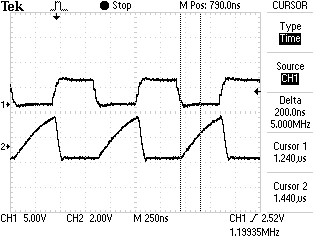
\includegraphics[width=\textwidth]{5.jpg}
\end{figure}
Schottky-dioden hindrer transistoren fra å gå i metning.
Da holder transistoren mindre ladningen og det går raskere å bytte modus.
